% digitalizace https://yangcha.github.io/iview/iview.html
%
%\usetikzlibrary{calc}
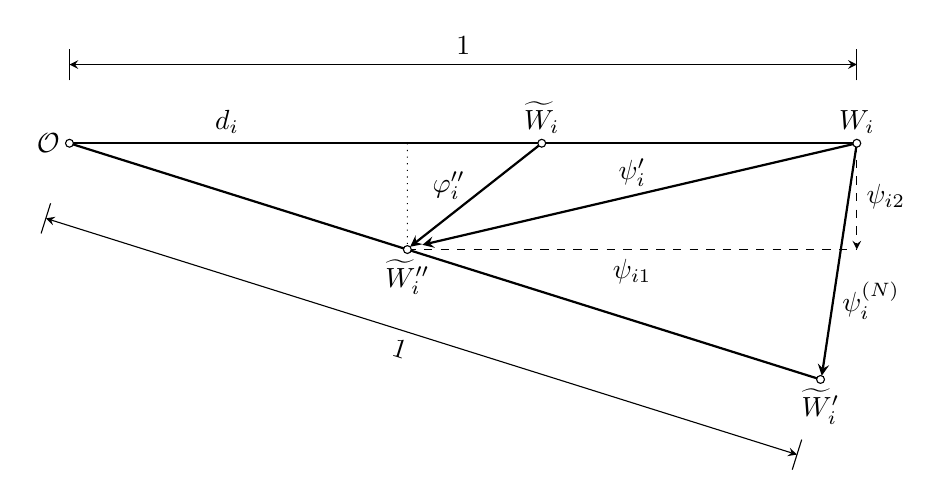
\begin{tikzpicture}[xscale=10,yscale=-10,>=stealth]
  \begin{scope}

    \def\dim{1.0000};            % dist unit
    \def\dc {0.0050};            % circle
    \def\cos{0.953939201416946}  % rotation 17.458 degrees
    \def\sin{0.300};

    \def\Ax{0};
    \def\Ay{0};
    \def\Bx{\dim};
    \def\By{0};
    \def\Fx{\dim*\cos};
    \def\Fy{\dim*\sin};
    \def\Cx{\dim/20*12};
    \def\Cy{\Ay};
    \def\Dx{\Fx/20.0*9};
    \def\Dy{\Fy/20.0*9}
    \def\Ex{\Bx};
    \def\Ey{\Dy};

    \coordinate (A) at (\Ax,\Ay);
    \coordinate (B) at (\Bx,\By);
    \coordinate (C) at (\Cx,\Cy);
    \coordinate (D) at (\Dx,\Dy);
    \coordinate (E) at (\Ex,\Ey);
    \coordinate (F) at (\Fx,\Fy);

    \begin{scope}
      \def\Gx{\Ax};
      \def\Gy{\Ay-0.1};
      \def\Hx{\Bx};
      \def\Hy{\By-0.1};
      \def\Kx{\Ax-0.1*\sin};
      \def\Ky{\Ay+0.1*\cos};
      \def\Lx{\Fx-0.1*\sin};
      \def\Ly{\Fy+0.1*\cos};

      \coordinate (G) at (\Gx,\Gy);
      \coordinate (H) at (\Hx,\Hy);
      \coordinate (K) at (\Kx,\Ky);
      \coordinate (L) at (\Lx,\Ly);

      \def\t{0.02}
      \draw[<->] (G)--(H);
      \draw[thin] (\Gx,\Gy+\t)--(\Gx,\Gy-\t);
      \draw[thin] (\Hx,\Hy+\t)--(\Hx,\Hy-\t);
      \node[above] at ({(\Gx+\Hx)/2},\Gy) {1};

      \draw[<->] (K)--(L);
      \draw[thin] (\Kx-\t*\sin,\Ky+\t*\cos)--(\Kx+\t*\sin,\Ky-\t*\cos);
      \draw[thin] (\Lx-\t*\sin,\Ly+\t*\cos)--(\Lx+\t*\sin,\Ly-\t*\cos);
      \node[below left,rotate=-17.458] at ({(\Kx+\Lx)/2},{(\Ky+\Ly)/2}) {1};
    \end{scope}

    \draw[thick] (A)--(B);
    \draw[thick] (A)--(F);

    \draw[thick, ->] (B)--(\Fx+\sin*\dc,\Fy-\cos*\dc);

    \draw[dashed, thin, ->] (B)--(E);
    \draw[thick, ->] (C)--(\Dx+0.707*\dc,\Dy-0.707*\dc);  % 0.707.. ~ sin(45)
    \draw[dashed, thin] (D)--(E);
    \draw[dotted] (\Dx,\Ay)--(D);
    \draw[thick, ->] (B)--(\Dx+\cos*4*\dc,\Dy-\sin*4*\dc);

    \draw[fill=white] (A) circle (\dc);
    \draw[fill=white] (B) circle (\dc);
    \draw[fill=white] (C) circle (\dc);
    \draw[fill=white] (D) circle (\dc);
    \draw[fill=white] (F) circle (\dc);

    \node[left]  at (A) {$\mathcal O$};
    \node[above] at (B) {$W_i$};
    \node[above] at (C) {$\widetilde W_i$};
    \node[below] at (D) {$\widetilde W_i''$};
    \node[below] at (F) {$\widetilde W_i'$};

    \node[above] at (0.2*\Bx,\Ay) {$d_i$};
    \node[left]  at ({(\Dx+\Cx)/2},{\Dy*0.40+\Cy*0.60}) {$\varphi_i''$};
    \node[above] at ({(\Dx+\Bx)/2},{(\Dy+\By)/2}) {$\psi_i'$};
    \node[below] at ({(\Dx+\Ex)/2},\Ey) {$\psi_{i1}$};
    \node[right] at (\Ex,{(\By+\Ey)/2}) {$\psi_{i2}$};
    \node[right] at ({(2*\Fx+\Bx)/3},{(2*\Fy+\By)/3}) {$\psi_i^{(N)}$};

  \end{scope}
\end{tikzpicture}

%
